\section{High-lift configuration}
The last case that was run is the McDonnel-Douglas 30P/30N three-element high-lift configuration. This case was only run with syn3D and the mesh is shown in~\Cref{fig:highmesh}. \Cref{tab:high} tabulates the free-stream conditions.
\begin{table}
    \centering
    \caption{Specification of free-stream flow conditions for the high-lift configuration}
    \label{tab:high}
    \begin{tabular}{ccc}
        \toprule
        $M_\infty$ & $\Rey \times 10^6$ & $\alpha$ (\degc)\\
        \midrule
        0.2 & 9 & 19 \\
        \bottomrule
    \end{tabular}
\end{table}
\begin{figure}
    \centering
    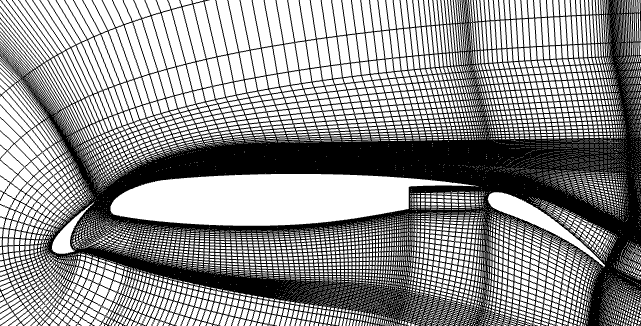
\includegraphics[width=0.7\textwidth]{figs/high/highlift}
    \caption{High-lift (syn3D): Close-up of the high-lift mesh.}
    \label{fig:highmesh}
\end{figure}
Unfortunately, this case could only be run on a mesh with an average $y^+$ of 50 and composed of around 100,000 elements. Of course, this is much too coarse of a mesh, especially for such a complex configuration, but the results are qualitatively accurate nonetheless.

\Cref{fig:highdist} shows a contour of the wall distance. \Cref{fig:highstream} depicts streamlines around the airfoils, which shows the expected recirculation regions.

\Cref{fig:highcp} compares the coefficient of pressure distribution with ISAAC~\cite{morrison1998numerical}. The cited reference also shows experimental data, although the results from ISAAC are virtually identical. It can be seen that the suction on the first element is not as pronounced as it should be for syn3D, which can be attributed to the coarseness of the grid. ISAAC also implements a transitional model, which allows the flow to naturally transition between the laminar regime and turbulent regime. Such a model is currently not implemented in syn3D, and this is another source of error~\cite{morrison1998numerical}. 

Finally, \Cref{tab:highld} compares the lift and drag coefficients. The lift coefficient is under-predicted and the drag coefficient is over-predicted. This discrepancy may be attributed to the reasons mentioned above.
\begin{figure}
    \centering
    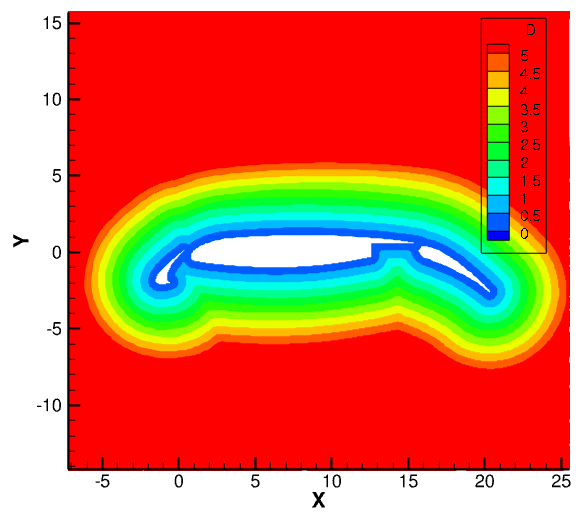
\includegraphics[width=0.7\textwidth]{figs/high/high_dist}
    \caption{High-lift (syn3D): Wall distance contour.}
    \label{fig:highdist}
\end{figure}
\begin{figure}
    \centering
    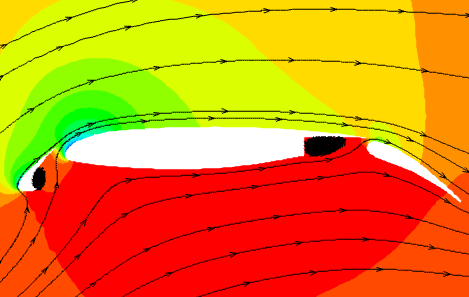
\includegraphics[width=0.7\textwidth]{figs/high/highstream}
    \caption{High-lift (syn3D): Streamlines around the high-lift configuration. Recirculation regions are identified by the solid black shapes.}
    \label{fig:highstream}
\end{figure}
\begin{figure}
    \centering
    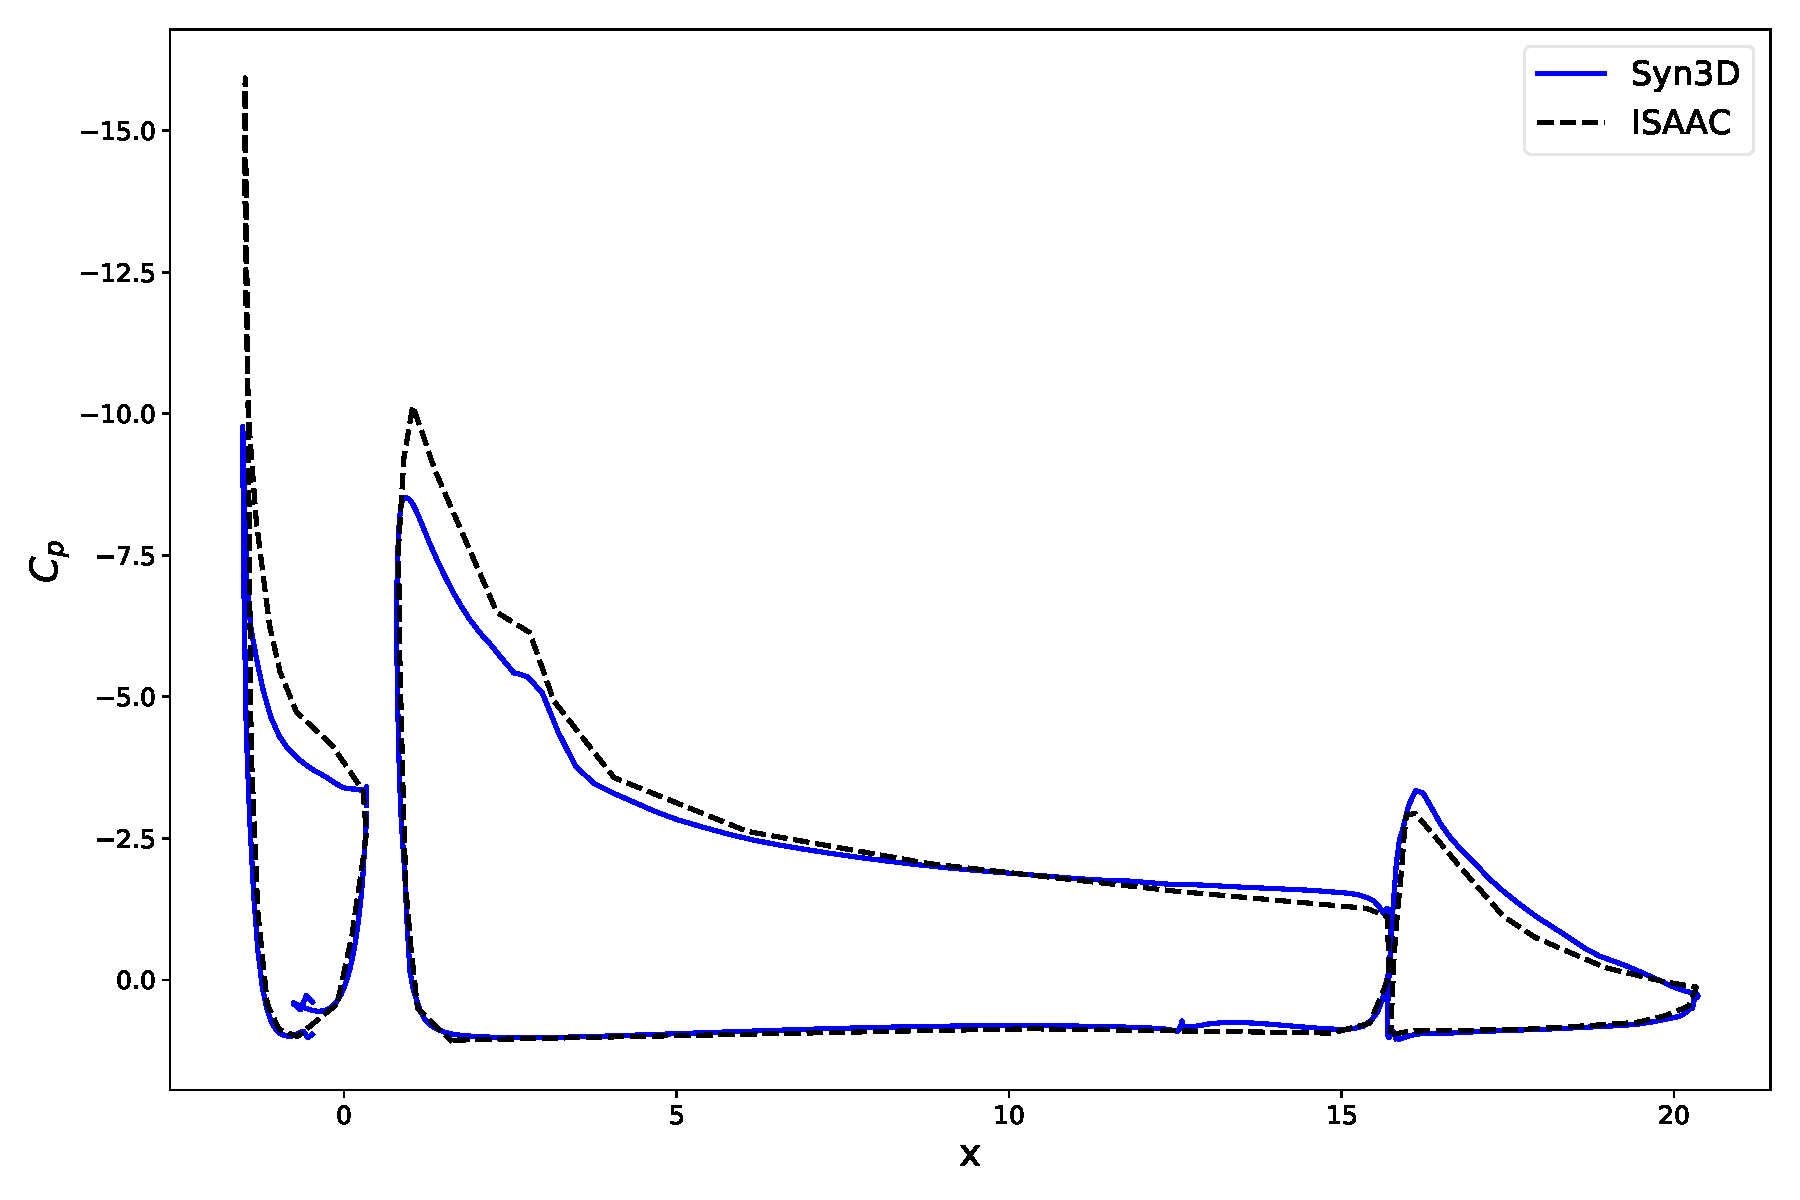
\includegraphics[width=0.95\textwidth]{figs/high/cp_highlift}
    \caption{High-lift (syn3D): Comparison of coefficient of pressure distribution.}
    \label{fig:highcp}
\end{figure}
\begin{table}
    \centering
    \caption{High-lift (syn3D): Comparison of lift and drag coefficients}
    \label{tab:highld}
    \begin{tabular}{l cc}
        \toprule
        Code & $C_L$ & $_D$ \\
        \midrule
        syn3D & 2.98 & 0.290\\
        ISAAC & $\approx$ 4 & $\approx$ 0.08\\
        \bottomrule
    \end{tabular}
\end{table}